\section{Introduction}
\label{sec:intro}

Mobile devices, edge, and cloud computing have the potential to form a \textit{computing continuum} on which new and disruptive types of applications can be built. %(Fig.~\ref{fig:continuum-overral}). 

This continuum enables the seamless convergence of heterogeneous infrastructure, stretching all the way from cloud resources to mobile devices, including intermediate steps such as ISP gateways, cellular base stations, and private cloud deployments.  

The heterogeneity of the computing continuum is profound and multi-faceted. In the cloud, computing resources are typically provided through virtualization and containerization~\cite{leitner2016patterns, Quatrocchi2016discrete}, and there is an illusion of infinite resource availability thanks to horizontal scaling. In contrast, in edge computing, computational resources are scarcer and must be managed very efficiently~\cite{Dehos14millimeter5g}~\cite{GarrigaMendonca2017}. This is even truer for mobile devices, as they are strongly constrained by battery limitations. 

In the cloud, networking protocols and technologies (e.g., traffic managers, DNS, etc.) allow clients to access resources across countries and continents. Conversely, in edge computing, in order to access resources they must be available within the client's network coverage, be it cellular (e.g., 5G) or local (e.g., domestic or office). Of course, we can consider a mobile device's computational resources  to be ``always available''.  

Finally, there are important QoS considerations that need to be made. While cloud resources can provide vast computing power through elasticity, accessing them may involve multiple hops of network communication, leading to prohibitive latency in the processing of client requests. Indeed, one of the main motivations for introducing edge computation is to mitigate the network latency~\cite{Shi:2016}, which is nullified when an execution is performed on the client's mobile device.

The advantage of embracing the computing continuum is that it allows an application to situationally and opportunistically decide where in the continuum a specific calculation should be performed. This decision will consider the resources that are actually available in the continuum at that specific moment in time, depending for example on the client's geo-location and connectivity, and will be informed by any existing QoS requirements, e.g., maximum acceptable latency~\cite{GuptaIfogSim17}. Given that the providers may not be able to coordinate and decide who should serve the client's request, this decision logic will need to be shared with the client's device, so that the best alternative can be selected every time.

In this paper, we propose a unified model for the computing continuum called A3-E. At its heart A3-E proposes a model for the automated management of a software service's life-cycle. The model takes its name from its four main phases: \textit{(A)wareness, (A)cquisition, (A)llocation} and \textit{(E)ngagement}. First of all, the model enables a mutual client-provider awareness that allows for the dynamic placement of stateless computation along the continuum. Second, the model extends the serverless computing paradigm~\cite{Hendrickson:2016,baldini2017serverless,GarrigaMendonca2017}, exploiting the function-as-a-service (FaaS) execution model~\cite{MateosFaaster17}, to allow stateless functions to be autonomously fetched, deployed and exposed by a provider. 

A3-E has been evaluated in the context of an Android-based augmented reality application. Thanks to A3-E the application was able to autonomously proxy its requests to services that were dynamically selected from a computing continuum. In our experiments the continuum was composed of a mobile runtime, a local-edge server, a (simulated) mobile-edge server in a cellular base station, and a cloud environment. The experiments show up to a 90\% reduction of latency when edge services are used instead of cloud services, and a 74\% decrease of battery consumption when computation is offloaded from the Android device to edge servers. 

The rest of this paper is organized as follows.  Section~\ref{sec:example} illustrates the continuum with a running scenario. Section~\ref{sec:proposal} provides a detailed description of the A3-E model, whereas Section~\ref{sec:implementation} details both the client-side implementation for Android platform and the server-side implementation for edge-computing. Section~\ref{sec:evaluation} reports on the experiments performed to evaluate our proposal with an augment reality application. Section~\ref{sec:related} presents related work. Finally, Section~\ref{sec:conclusions} concludes the paper and delineates future work.

\section{Running Example}
\label{sec:example}

\begin{figure}[tbp]
	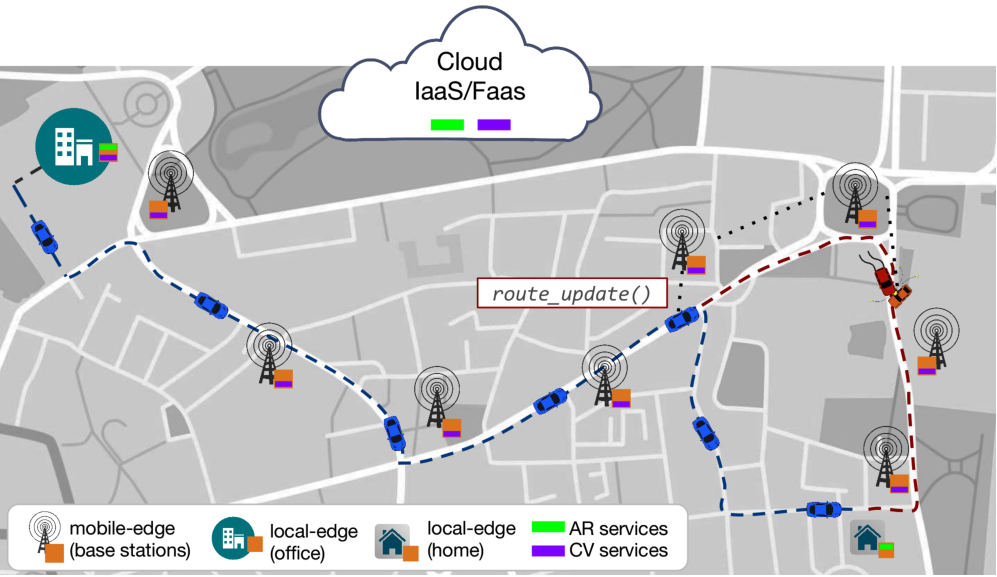
\includegraphics[width=0.9\textwidth]{figs/Continuum-Scenario}
	\caption{Heterogeneous applications such as Augmented Reality (AR) and Autonomous Vehicles (AV) interact with services deployed along the computational continuum (cloud, mobile-edge, local-edge, and mobile)}
	\label{fig:continuum-scenario}
\end{figure}

%Throughout this section an example scenario (Fig.~\ref{fig:continuum-scenario}) is used to illustrate the use of A3-E model and the cloud-edge-mobile continuum with different applications employed by a person with visual impairment.
We illustrate the computational continuum in an example scenario that starts in a user's office and finishes at her home. It involves different applications that rely on services executed in the cloud, edge, or in the user's own devices. 

First, let us assume the existence of a local-edge server in the user's office (hereafter called \textit{local-edge}). This server is owned by the company, and it is used to extend the computational capabilities of the devices operated by its employees. In our example, the user makes use of an AR application to craft virtual 3D objects that are added to her desk table. This application involves heavyweight image processing for the extraction of features from the captured scenes, as well as a trained neural network model to identify objects from a set of features. With the offloading of both tasks to the local-edge, the user can avoid recharging her glasses and can improve her productivity. Also, the additional storage on the edge servers allows a larger set of objects to be recognized, thanks to a more completely trained model.

After work, the user leaves her offices and enters her autonomous vehicle (AV). During her way home, the vehicle makes use of services deployed at edge servers located at cellular base stations (hereafter called \textit{mobile-edge}) to receive low-latency updates about the best plan to reach her destination. This way, within milliseconds the vehicle can be suggested to adjust its routes to avoid heavy traffic. In particular, let's say that a new path consists of residential streets without mobile-edge coverage. The AV continues to fetch updates, which are now served by a cloud provider. The additional network latency is compensated with the low speed limit of the residential area.

Finally, at home the user can start using her domestic local-edge server. She finds out about a new mobile game application. Upon installation, the local-edge server becomes aware of a new continuum-compliant application and, while the app continues to run locally on her device, it proceeds to setup the services needed to allow the application to offload some of the computation. Once the setup is complete, the application autonomously starts using the edge services with the purpose of preserving the device's resources. Not only does the game's performance improve, battery consumption is also reduced.  

This scenario exploits different parts of the continuum. Cloud services are employed as a reliable alternative to edge services. Similarly, local services are employed as alternatives to edge services until they have been acquired and made available by a local-edge server. Whilst the transition between mobile-edge and cloud was transparent, the use of local-edge services involved the mutual client-server awareness.

